\documentclass{beamer}

\usepackage{beamerthemesplit}
\usepackage{amsmath}
\usepackage{amsfonts}
\usepackage{amssymb}
\usepackage{qtree}
\usepackage{cancel}
\usepackage{tkz-graph}
%\usepackage[pdftex]{graphicx}

\mode<presentation>
{
  \usetheme{Warsaw}
  % or ...

  %\setbeamercovered{transparent}
  % or whatever (possibly just delete it)
}


\usepackage[english]{babel}
% or whatever

\usepackage[latin1]{inputenc}
% or whatever

\usepackage{times}
\usepackage[T1]{fontenc}

\title{Probabilistic Logical Networks}

\subtitle{Introduction}

\author{Nil Geisweiller}

\institute[OpenCog Foundation] % (optional, but mostly needed)
{
  OpenCog Foundation
}

\date[The Robotics Garage Project 2016] % (optional, should be abbreviation of conference name)
{The Robotics Garage Project 2016}


\AtBeginSection[]
{
  \begin{frame}<beamer>{Outline}
    \tableofcontents[currentsection,currentsection]
  \end{frame}
}

\AtBeginSubsection[]
{
  \begin{frame}<beamer>{Outline}
    \tableofcontents[currentsection,currentsubsection]
  \end{frame}
}

%\newcommand{\AND}{\textit{AND}}
%\newcommand{\OR}{\textit{OR}}
%\newcommand{\NOT}{\textit{NOT}}
\newcommand{\AND}{\land}
\newcommand{\OR}{\lor}
\newcommand{\NOT}{\lnot}


\begin{document}

\frame
{
  \maketitle
}
\section[Outline]{}
\frame{\tableofcontents}

\section{Introduction}

\frame
{
  \frametitle{What is PLN?}

  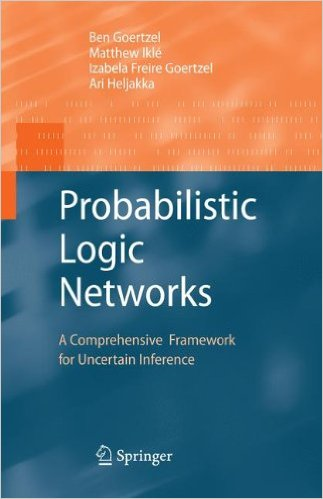
\includegraphics[scale=0.3]{PLN.jpg}\\
  {\scriptsize
    {\color{green}http://wiki.opencog.org/wikihome/index.php/OpenCogPrime:PLNBookErrata}\\
    {\color{green}http://wiki.opencog.org/wikihome/index.php/PLNBook}}
}

\frame
{
  \frametitle{What is PLN?}

  \begin{itemize}
  \item Handling the kind of \alert{uncertain, messy reasoning}
    we humans are so good at, but machines not so good.
  \item While maintaining full consistency with
    \alert{Probability Theory}!\\
    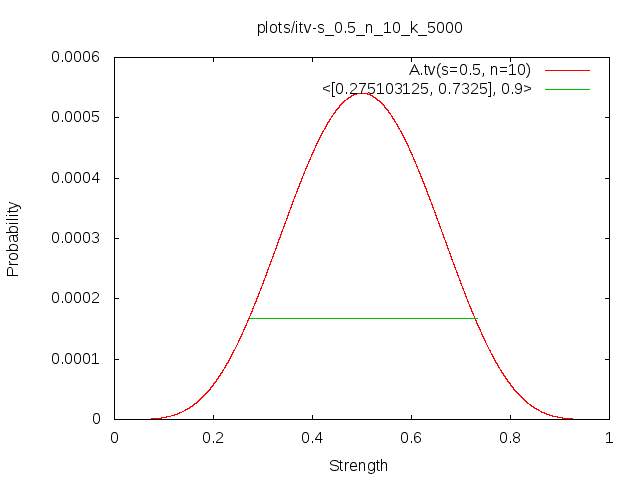
\includegraphics[scale=0.3]{dtv-n10.png}
    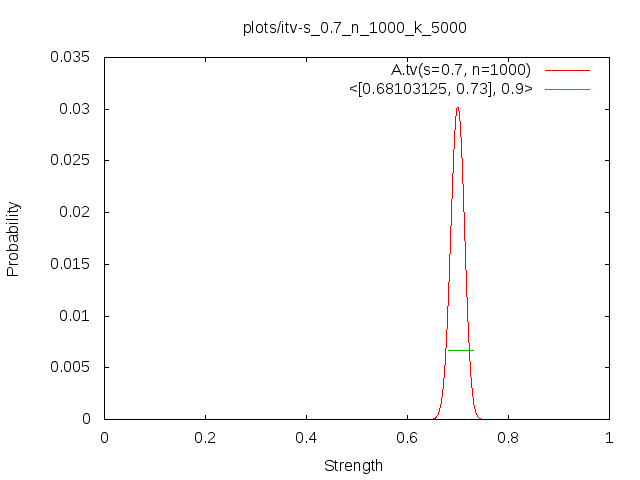
\includegraphics[scale=0.3]{dtv-n1000.png}
  \end{itemize}
}

\frame
{
  \frametitle{What is PLN?}

  Follow the {\color{red}Patternist Philosophy}. Mixing {\color{red}extensional}
  and {\color{red}intensional} reasoning.\\
  \begin{columns}
    \column{1.5in}
    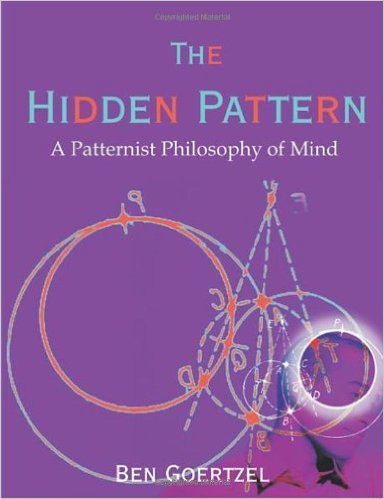
\includegraphics[scale=0.3]{pattern_philosophy.jpg}
    \column{1.5in}
    Inheritance <0.4, 0.8>\\
      $\ \ \ $Dolphin\\
      $\ \ \ $Fish
  \end{columns}
}

\frame
{
  \frametitle{What is PLN?}

  Very good at mixing knowledge coming from {\color{red}different
    sources} with {\color{red}different confidence levels}.\\[1cm]
  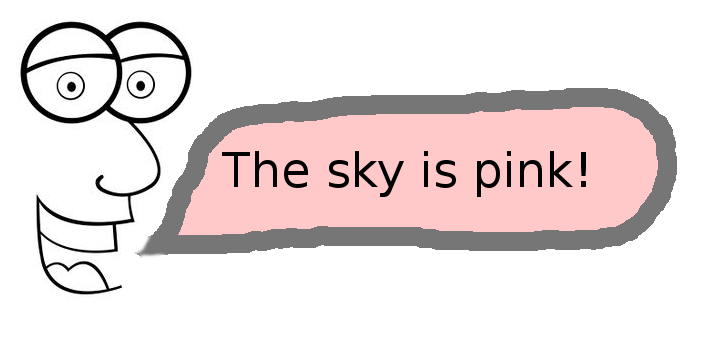
\includegraphics[scale=2.2]{Pink.png} 
\includegraphics[scale=0.11]{Blue.png}
}

\section{Example}

\frame
{
  \frametitle{Example: Query}
  
  \underline{\alert{{\it What is the color of the sky?}}}\\[.5cm]

  Inheritance <?>\\
  $\ \ \ $Sky\\
  $\ \ \ $Variable "\$Color"\\
}

\frame
{
  \frametitle{Example: Background Knowledge}

  {\tiny
  \begin{columns}
    \column{1.5in}
    \underline{\alert{{\it John says that the sky is Pink}}} (KB.1)\\[.2cm]
    Evaluation <1 0.99>\\
    $\ \ \ $Predicate "Say"\\
    $\ \ \ $List\\
    $\ \ \ $$\ \ \ $Concept "John"\\
    $\ \ \ $$\ \ \ $Inheritance\\
    $\ \ \ $$\ \ \ $$\ \ \ $Concept "Sky"\\
    $\ \ \ $$\ \ \ $$\ \ \ $Concept "Pink"\\[.5cm]

    \underline{\alert{{\it John's credential is low}}} (KB.2)\\[.2cm]
    Implication <0.6 0.1>\\
    $\ \ \ $Variable "\$X"\\
    $\ \ \ $Evaluation\\
    $\ \ \ $$\ \ \ $Predicate "Say"\\
    $\ \ \ $$\ \ \ $List\\
    $\ \ \ $$\ \ \ $$\ \ \ $John\\
    $\ \ \ $$\ \ \ $$\ \ \ $Variable "\$X"\\
    $\ \ \ $Variable "\$X"\\

    \column{1.5in}

    \underline{\alert{{\it According to my limited observations the sky is
        blue}}} (KB.3)\\[.2cm]
    Inheritance <0.9 0.6>\\
    $\ \ \ $Concept "Sky"\\
    $\ \ \ $Concept "Blue"\\[.5cm]

    \underline{\alert{{\it Though sometimes pink as well}}} (KB.4)\\[.2cm]
    Inheritance <0.1 0.6>\\
    $\ \ \ $Concept "Sky"\\
    $\ \ \ $Concept "Pink"\\[.5cm]

\end{columns}
}
}

\frame
{
  \frametitle{Example: Rules}
  
  {\tiny
  \begin{columns}
    
    \column{1.5in}
    
    \underline{\alert{{\it Deduction}}} (R.1)\\[.2cm]
    Inheritance <TV1>\\
    $\ \ \ $A\\
    $\ \ \ $B\\
    Inheritance <TV2>\\
    $\ \ \ $B\\
    $\ \ \ $C\\
    $\vdash$\\
    Inheritance <$f_1$(TV1, TV2, ...)>\\
    $\ \ \ $A\\
    $\ \ \ $C\\[.5cm]

    \underline{\alert{{\it Disjunction Composition}}} (R.2)\\[.2cm]
    P <TV1>\\
    Q <TV2>\\
    $\vdash$\\
    And <$f_4$(TV1, TV2)>\\
    $\ \ \ $P\\
    $\ \ \ $Q\\

    \column{1.5in}

    \underline{\alert{{\it Inversion}}} (R.3)\\[.2cm]
    Inheritance <TV>\\
    $\ \ \ $A\\
    $\ \ \ $B\\
    $\vdash$\\
    Inheritance <$f_3$(TV, ...)>\\
    $\ \ \ $B\\
    $\ \ \ $A\\[.5cm]

    \underline{\alert{{\it Conditional Instantiation}}} (R.4)\\[.2cm]
    Implication <TV>\\
    $\ \ \ $V\\
    $\ \ \ $P\\
    $\ \ \ $Q\\
    T\\
    $\vdash$\\
    Q[V->T] <$f_2$(TV, ...)>\\

  \end{columns}

  }
}

\frame
{
  \frametitle{Example: Inference}

  {\small
    Only one inference step: \alert{Apply} (R.4) on (KB.2)\\[.2cm]
    Inheritance <0.6 0.099>\\
    $\ \ \ $Concept "Sky"\\
    $\ \ \ $Concept "Blue"\\[.5cm]
    
    When producing that conclusion PLN will \alert{merge} it
    to the existing one which has a much higher confidence, so the
    result will be\\[.2cm]
    Inheritance <0.91 0.62>\\
    $\ \ \ $Concept "Sky"\\
    $\ \ \ $Concept "Blue"\\[.5cm]
  }
}

\section{Bottom Up}

\subsection{Level 0: Subset, And, Or, Not}

\frame
{
  \frametitle{SubSet}

  \begin{columns}
    \column{1.5in}
    
    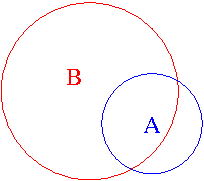
\includegraphics[scale=0.7]{subset_A_B.pdf}

    \column{1.5in}

    
\includegraphics[scale=0.25]{Fuzzy_SubSet_A_B.png}

  \end{columns}

    SubSet {\color{blue}A} {\color{red}B} <s c>
    $\ \equiv\ P({\color{red}B}|{\color{blue}A})=s$\\[2ex]

  \begin{itemize}
  \item
    Fuzzy/Multi sets
  \end{itemize}

  \begin{eqnarray*}
    P({\color{red}B}|{\color{blue}A})
    &
    =
    &
    \frac{\sum_x \min({\color{blue}A}(x), {\color{red}B}(x))}
    {\sum_x {\color{blue}A}(x)}
  \end{eqnarray*}

}

\frame
{
  \frametitle{And, Or, Not}

  \begin{itemize}
    \item 
      % \begin{columns}
        % \column{1.5in}
        And <$P(A, B)\ c$>\\
        $\ \ \ $A\\
        $\ \ \ $B\\[.5cm]
        % \column{1.5in}
        % $P(A)\times P(B)$\\
      % \end{columns}
    \item 
      Or <$P(A \cup B)\ c$>\\
      $\ \ \ $A\\
      $\ \ \ $B\\[.5cm]
    \item 
      Not <$P(\lnot A)\ c$>\\
      $\ \ \ $A\\
      $\ \ \ $B\\
  \end{itemize}
}

\frame
{
  \frametitle{Level 0: Subset, And, Or, Not}

  Level 0 is all about \alert{extensional} constructs.\\[.25cm]
  
  Rules dealing with these constructs
  \begin{itemize}
    \item modus ponens
    \item deduction, inversion
    \item conjunction, disjunction, negation compositions
    \item universal and conditional instantiations
  \end{itemize}
  form the \alert{basis of PLN}.\footnote{ForAll let aside}\\[.25cm]

  \pause

  \begin{beamerboxesrounded}{Take away}
    All the remaining of PLN is built on top of that.
  \end{beamerboxesrounded}

}

\subsection{Level 1: Extensional Inheritance and Implication}

\frame
{
  \frametitle{SubSet $\equiv$ Extensional Inheritance}

  \begin{columns}
    \column{2in}

    ExtensionalInheritance <TV>\\
    $\ \ \ $A\\
    $\ \ \ $B\\

    \column{.5in}
    
    $\equiv$
    
    \column{1.2in}
  
    SubSet <TV>\\
    $\ \ \ $A\\
    $\ \ \ $B\\
  \end{columns}
}

\frame
{
  \frametitle{Extensional Inheritance $\equiv$ Extensional
    Implication}

  \begin{columns}
    \column{2in}

    ExtensionalInheritance <TV>\\
    $\ \ \ $SatisfyingSet P\\
    $\ \ \ $SatisfyingSet Q\\

    \column{.1in}
    
    $\equiv$
    
    \column{2in}
  
    ExtensionalImplication <TV>\\
    $\ \ \ $P\\
    $\ \ \ $Q\\
  \end{columns}

  $\ $\\[1cm]
  
  \pause

  \begin{columns}
    \column{2in}

    Member <TV>\\
    $\ \ \ $T\\
    $\ \ \ $SatisfyingSet P\\

    \column{.1in}
    
    $\equiv$
    
    \column{2in}
  
    Evaluation <TV>\\
    $\ \ \ $P\\
    $\ \ \ $T\\
  \end{columns}

}

\subsection{Level 2: Intensional Inheritance and Implication}

\frame
{
  \frametitle{Intensional Inheritance $\equiv$ Extensional Inheritance}

  Intensional Inheritance $\equiv$ Extensional Inheritance\footnote{in
    pattern space}!!!\\[.5cm]

  \pause
  
  \begin{columns}
    \column{1.9in}

    IntentionalInheritance <TV>\\
    $\ \ \ $A\\
    $\ \ \ $B\\

    \column{.05in}
    
    $\equiv$
    
    \column{2in}
  
    ExtensionalInheritance <TV>\\
    $\ \ \ $Patterns A\\
    $\ \ \ $Patterns B\\
  \end{columns}

  $\ $\\[0.5cm]

  \begin{beamerboxesrounded}{Patterns A}
    All \alert{properties} of A (super-sets) weighted by a
    \alert{prior} (Solomonoff Universal Distribution).
  \end{beamerboxesrounded}

}

\iffalse

\frame
{
  \frametitle{What is a property?}

  \begin{center}
    %\alert{
      Property = Super-set
    %}

      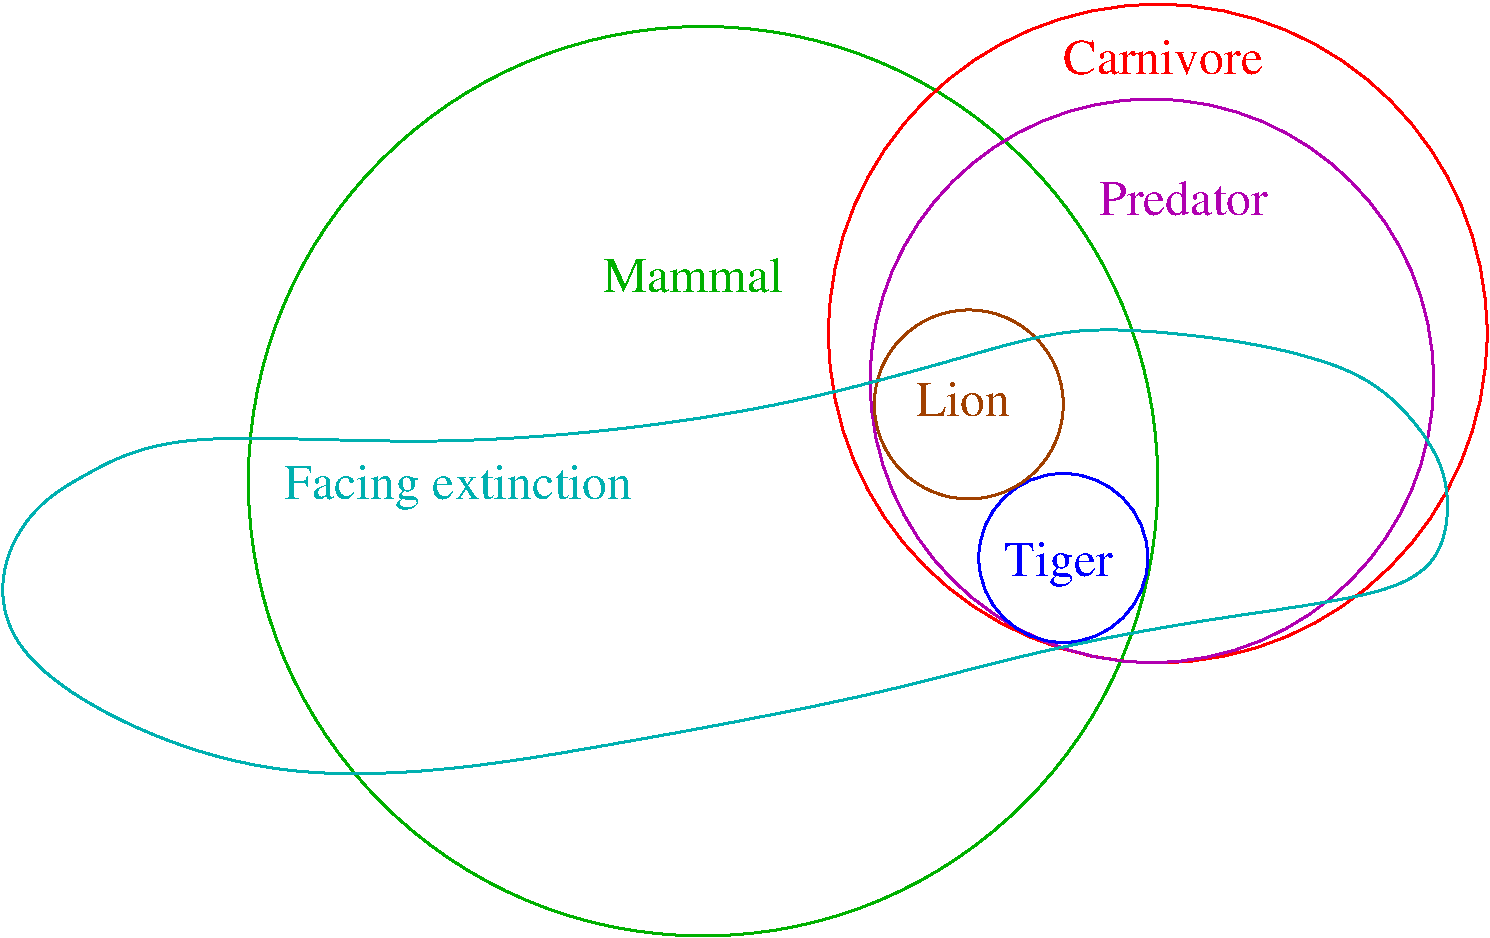
\includegraphics[scale=0.35]{property_superset.pdf}
  
  \end{center}

%   \pause

%   \begin{itemize}
%   \item<+-> Properties of Tiger: Predator,
%  Carnivore, Facing extinction, Mammal
%   \end{itemize}
}

\frame
{
  \frametitle{What is a property?}

  \begin{columns}

    \column{2in}
    
    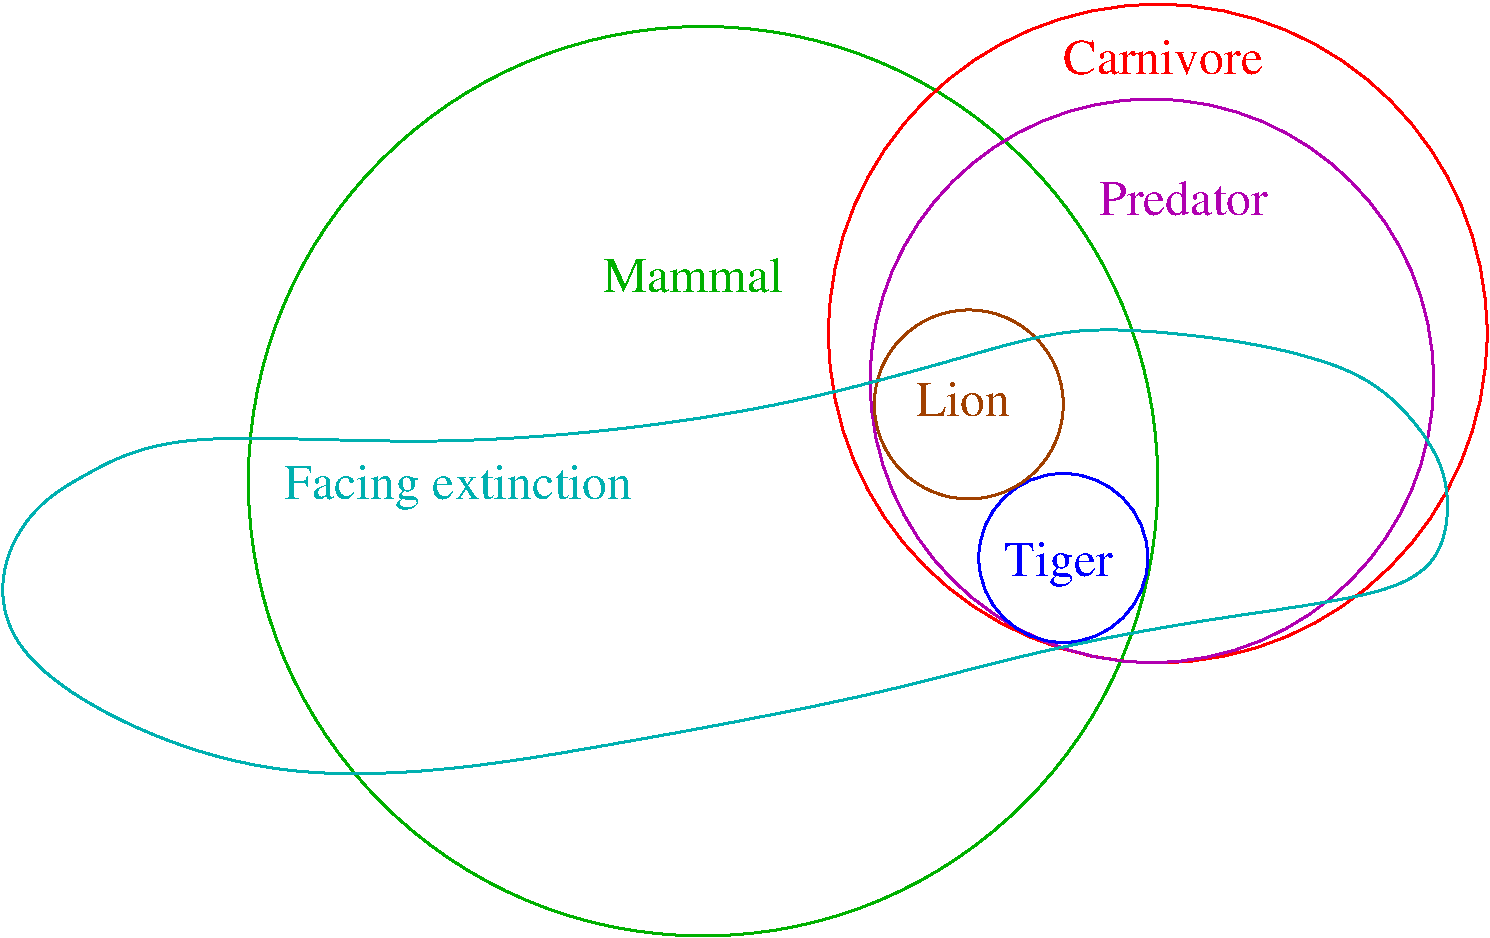
\includegraphics[scale=0.2]{property_superset.pdf}
    
    \column{2in}
  
    {\footnotesize
      \begin{itemize}
      \item {\tt SubSet {\color{blue}T} {\color{cyan}Fe} <1>}
      \item {\tt SubSet {\color{blue}T} {\color{purple}P} <1>}
      \item {\tt SubSet {\color{blue}T} {\color{red}C} <1>}
      \item {\tt SubSet {\color{blue}T} {\color{green}M} <1>}
      \item {\tt SubSet {\color{brown}L} {\color{cyan}Fe} <0.8>}
      \item {\tt SubSet {\color{brown}L} {\color{blue}T} <0>}
      \end{itemize}
    }
  \end{columns}

   \pause

   \begin{columns}

     \column{1.3in}

     {\footnotesize
     \begin{itemize}
     \item $P({\color{cyan}Fe}|{\color{blue}T})=1$
     \item $P({\color{purple}P}|{\color{blue}T})=1$
     \item $P({\color{red}C}|{\color{blue}T})=1$
     \item $P({\color{green}M}|{\color{blue}T})=1$
     \item $P({\color{cyan}Fe}|{\color{brown}L})=0.8$
     \item $P({\color{blue}T}|{\color{brown}L})=0$
     \end{itemize}
     }

     \pause

     \column{0.2in}

     $\Rightarrow$

     \column{2in}

     \begin{beamerboxesrounded}{$F$ is a \alert{property} of $G$ if}
       \alert{$P(F|G)$} is sufficiently \alert{high}
     \end{beamerboxesrounded}

   \end{columns}
}

\frame
{
  \frametitle{What is an \alert{interesting} property?}

  But potentially$\ldots$
  \alert{infinity of super-sets} (i.e. properties) of a term\\[5ex]

  \begin{beamerboxesrounded}{Interesting property of a term}
    \begin{enumerate}
    \item Help \alert{differentiate} that term
    \item \alert{Less complex} than the term itself
    \end{enumerate}
  \end{beamerboxesrounded}
}

\frame
{
  \frametitle{Interesting property: help \alert{differentiate}}

  %Example with the property 
  \alert{$being\_part\_of\_the\_universe$}\\
  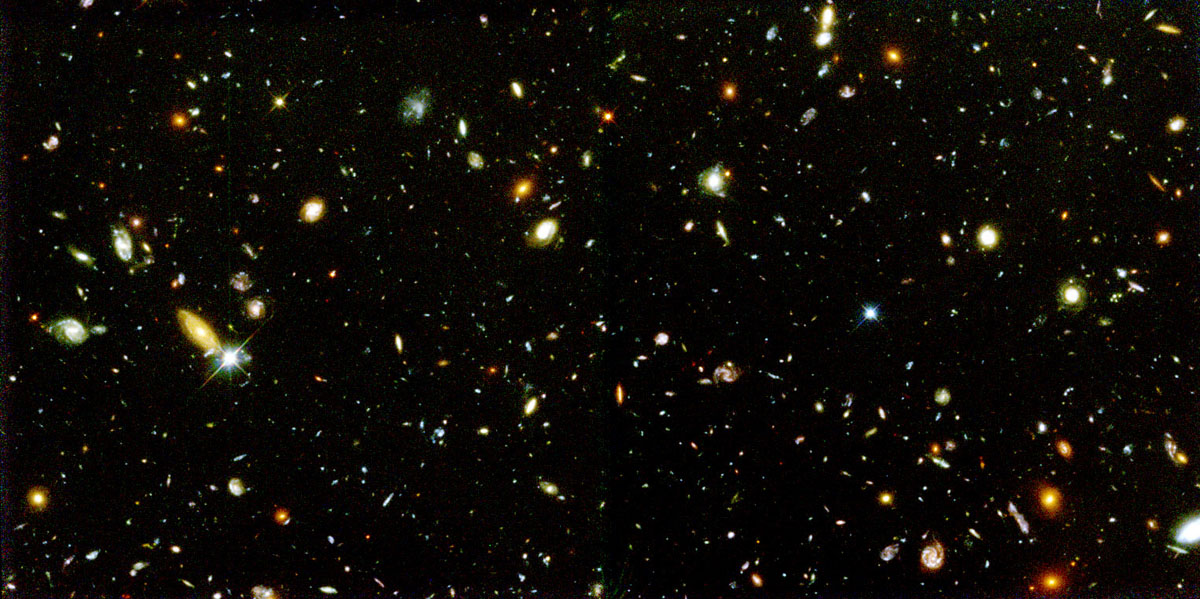
\includegraphics[scale=0.12]{universe.jpg}

  $P(being\_part\_of\_the\_universe|Tiger)=1$\\
  $P(being\_part\_of\_the\_universe|Lion)=1$\\
  $P(being\_part\_of\_the\_universe|Chair)=1$\\
  $\ldots$\\

  \pause

  \begin{beamerboxesrounded}{being\_part\_of\_the\_universe
      \alert{not interesting property} of Tiger}
    because it does not help to differentiate it in any manner
  \end{beamerboxesrounded}
}

\frame
{
  \frametitle{Interesting property: help \alert{differentiate}}

  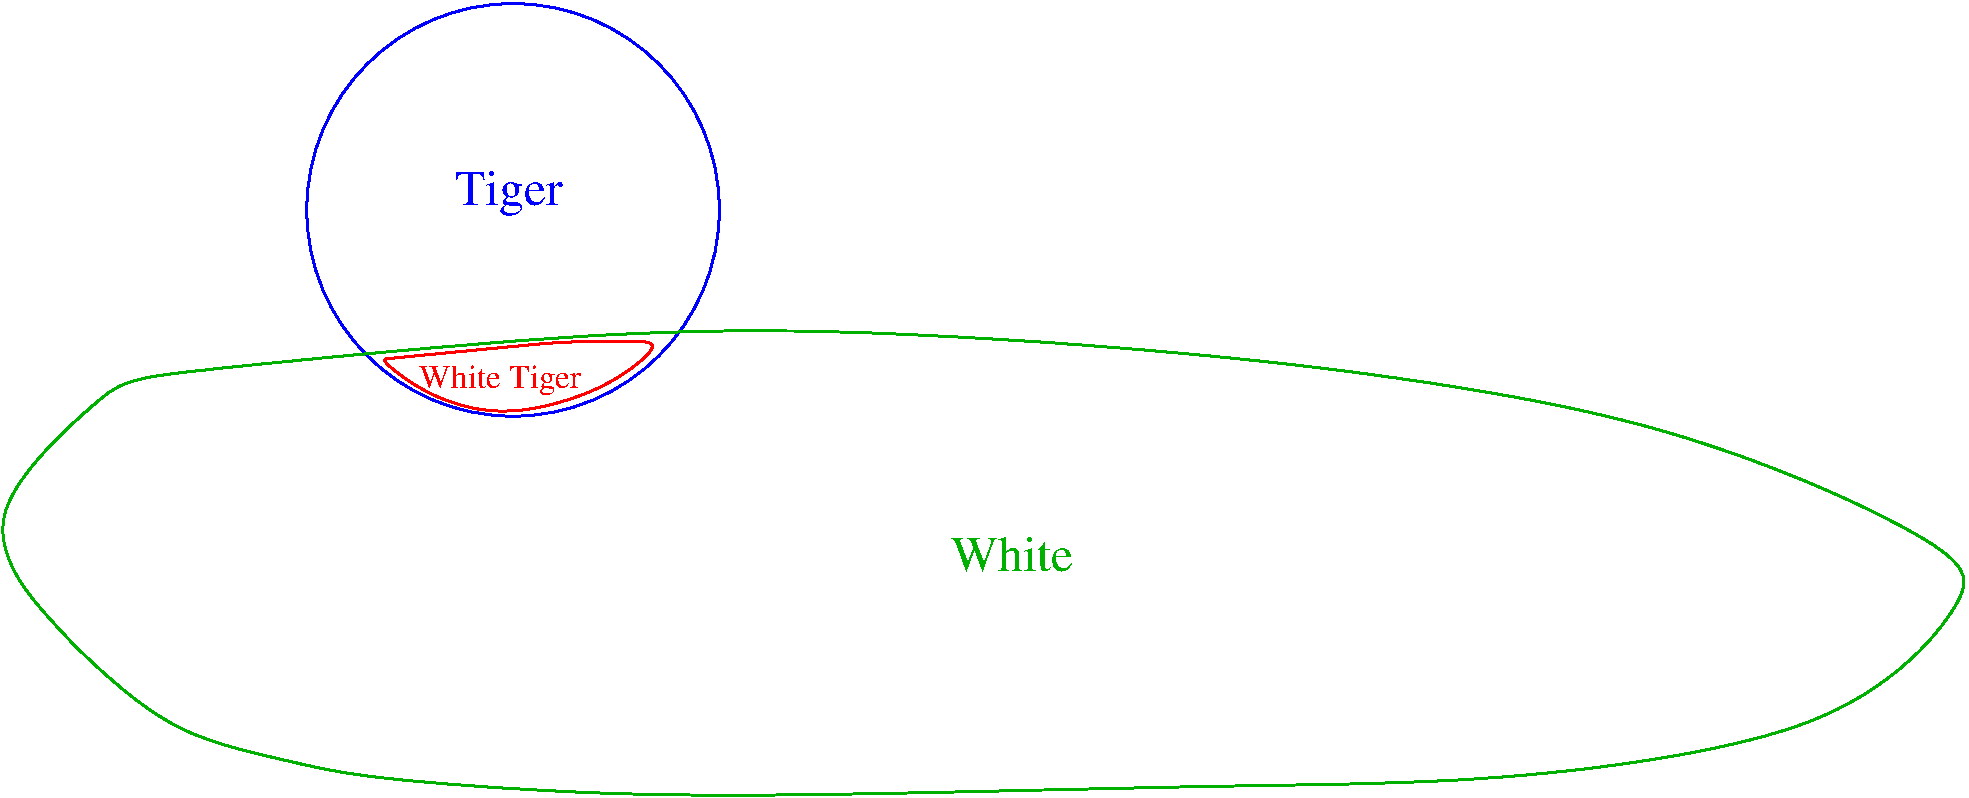
\includegraphics[scale=0.32]{white_tiger.pdf}

  \begin{beamerboxesrounded}{White is an
      \alert{interesting property} of White\_Tiger}
    \begin{itemize}
    \item $P({\color{green}White}|{\color{red}White\_Tiger})=1$
    \item $P({\color{green}White}|Golden\_Tiger)=0$
%    \item $White\ AND\ Tiger = White\_Tiger$
    \end{itemize}
  \end{beamerboxesrounded}
 
}

\frame
{
  \frametitle{Interesting property: help \alert{differentiate}}

  \begin{beamerboxesrounded}{$F$ helps \alert{differentiate} $G$,
      or $F$ is \alert{associated} with $G$ iff}
    $P(F|G) > P(F|\lnot G)$
  \end{beamerboxesrounded}
  
  \[ASSOC(F,G) = [P(F|G)-P(F|\lnot G)]^+\]

  \pause

  Examples
  \begin{enumerate}
  \item<+-> 
    $\alert{ASSOC(being\_part\_of\_the\_universe, Tiger)}$\\
    $
    \begin{array}{clrl}
      = & & [ & P(being\_part\_of\_the\_universe|Tiger)\\
      & &  & - P(being\_part\_of\_the\_universe|\lnot Tiger)]^+\\
      = & [1-1]^+ & = & \alert{0}\\
    \end{array}
    $
  \item<+->
    $\alert{ASSOC(White,White\_Tiger)}$\\
    $
    \begin{array}{cl}
      = & [ P(White|White\_Tiger) - P(White|\lnot White\_Tiger)]^+\\
      = & [ 1 - 0.3 ]^+ = \alert{0.7}
    \end{array}
    $
  \end{enumerate}

}

\frame
{
  \frametitle{Interesting property: \alert{Less complex} than the term itself}
  
  \only<1>{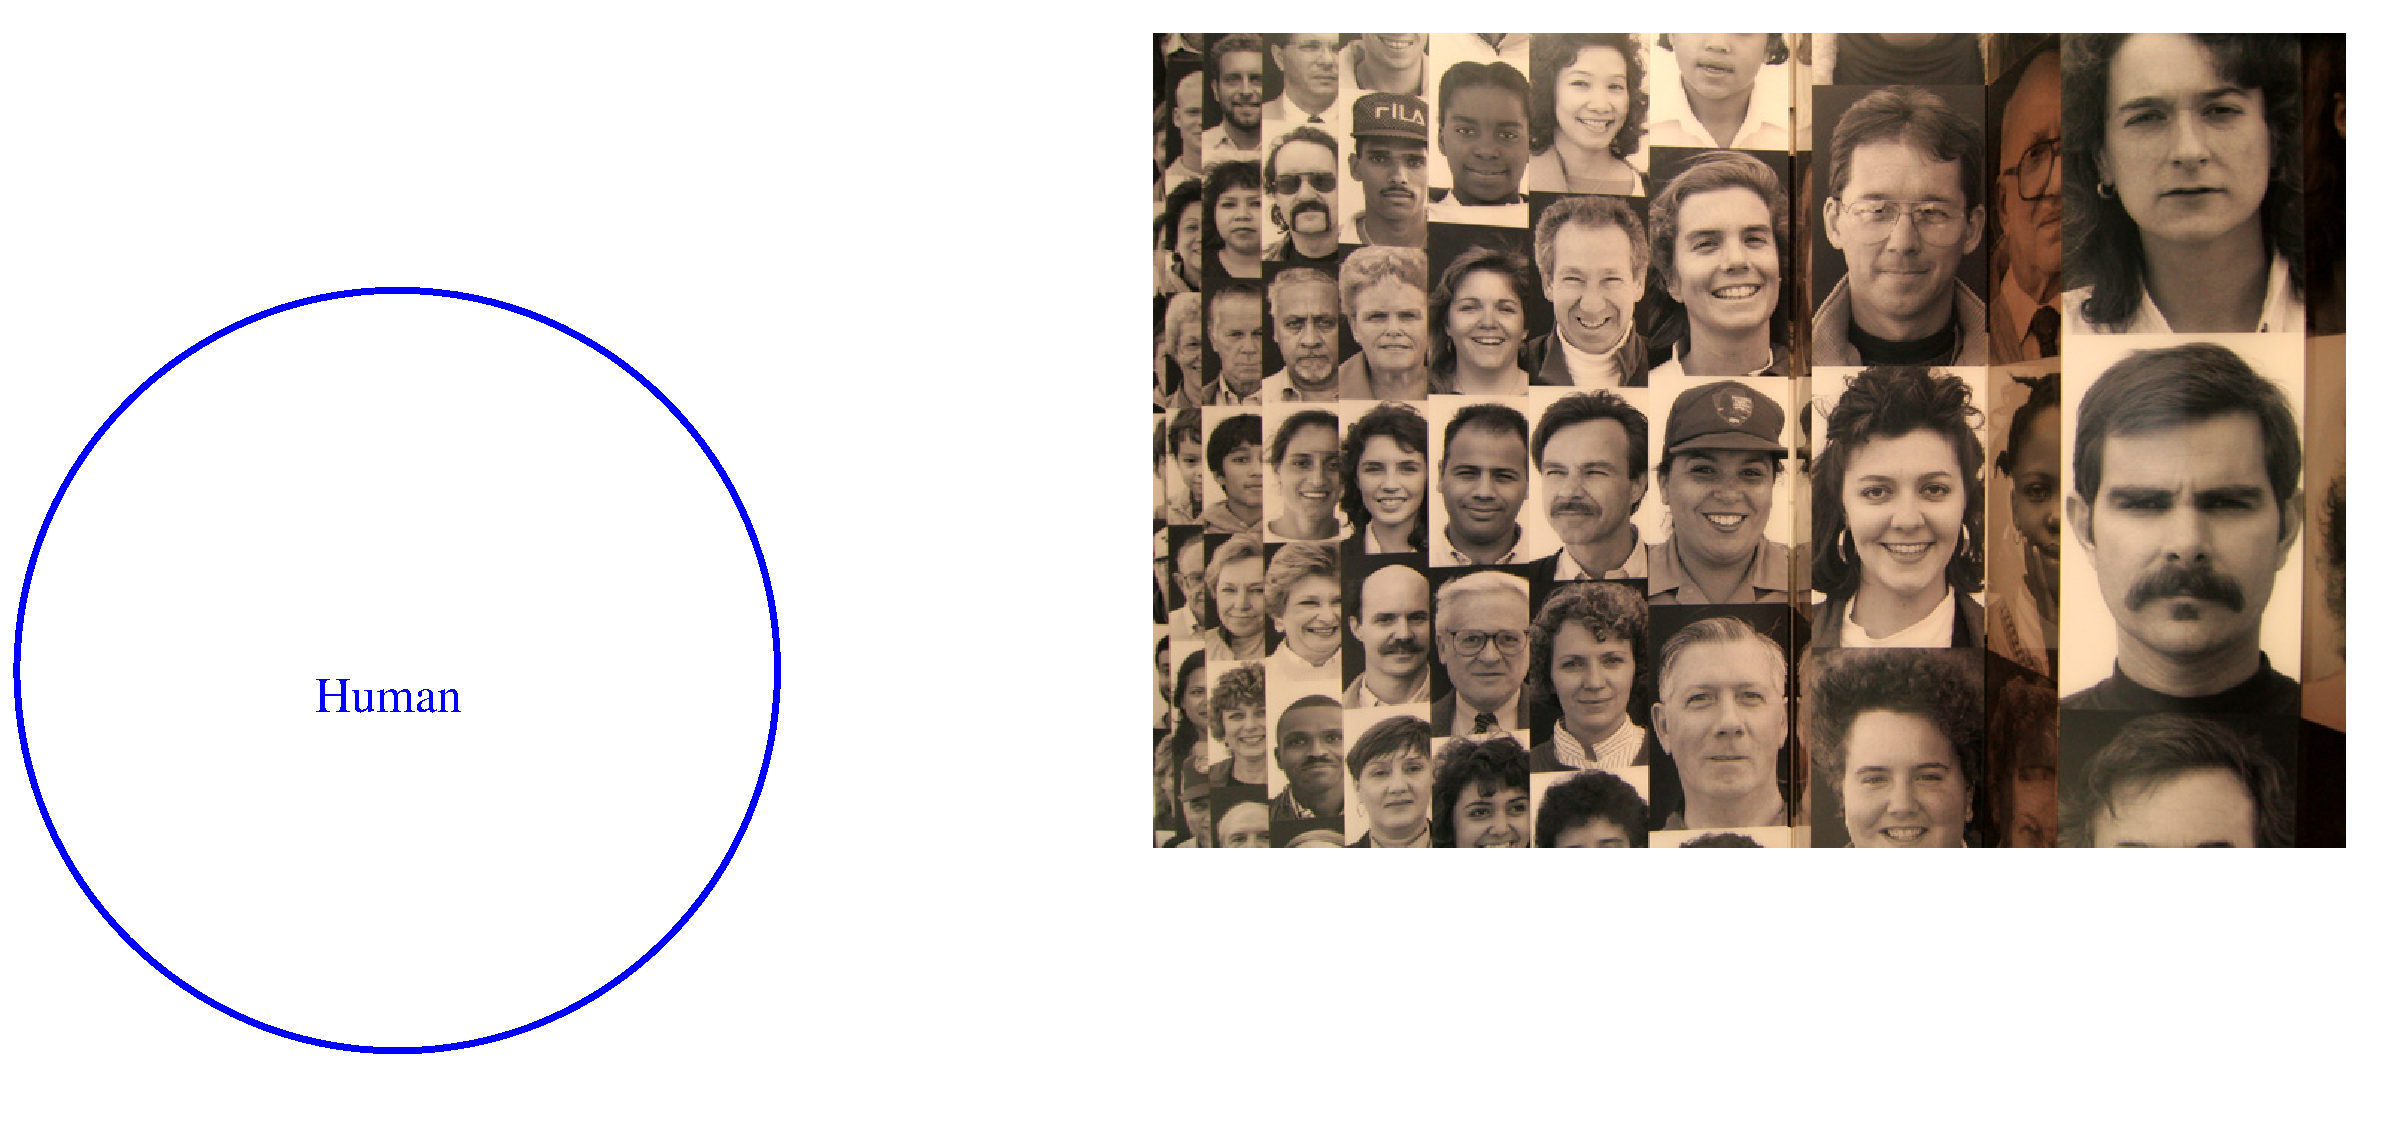
\includegraphics[scale=0.25]{human_chair_pic1.pdf}}
  \only<2>{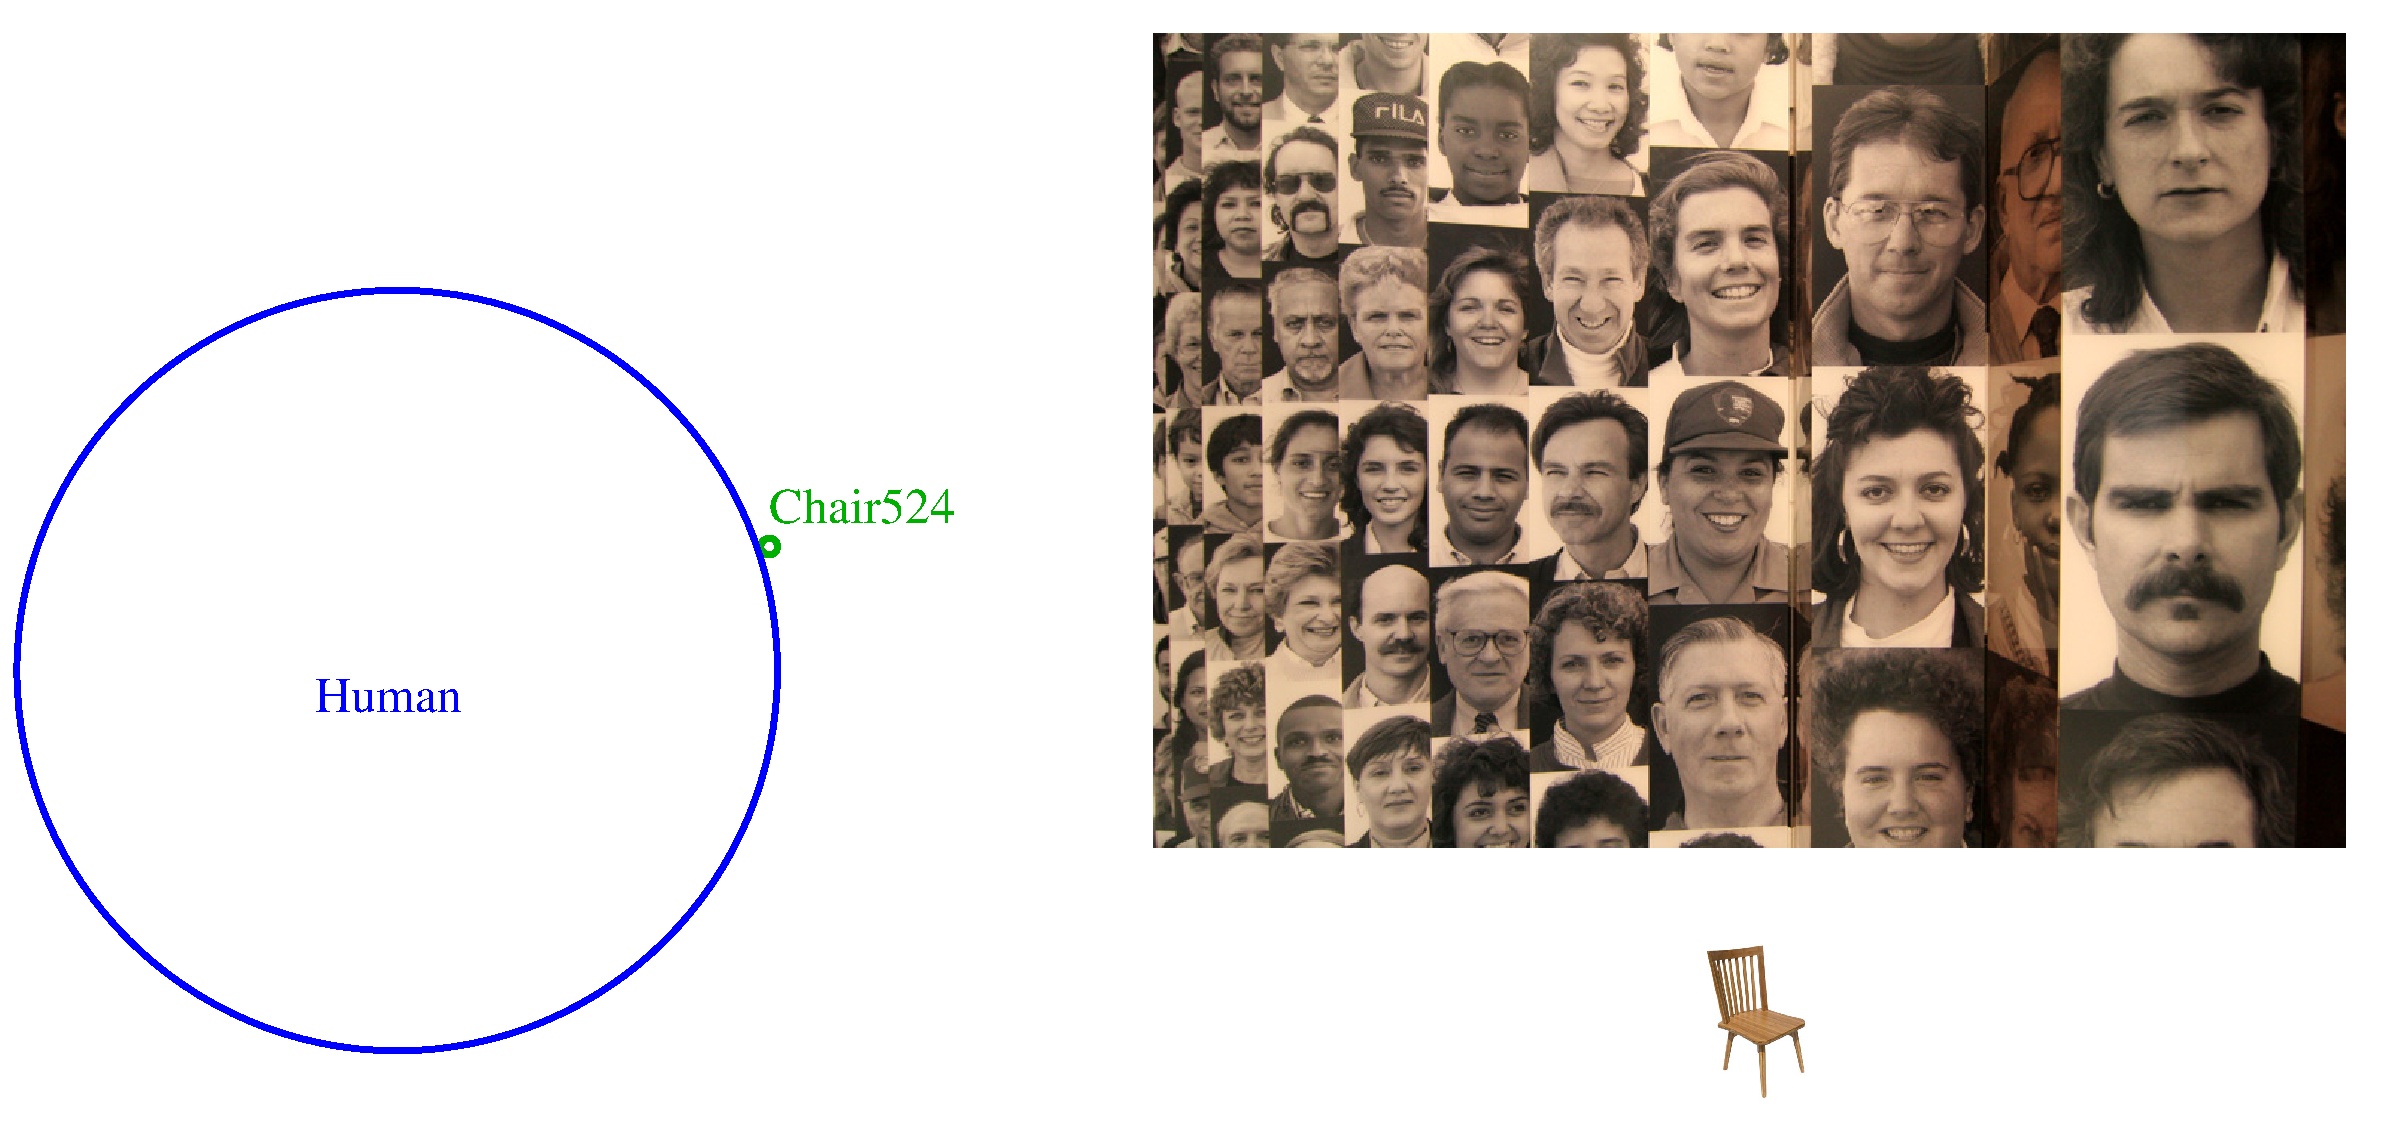
\includegraphics[scale=0.25]{human_chair_pic2.pdf}}
  \only<3->{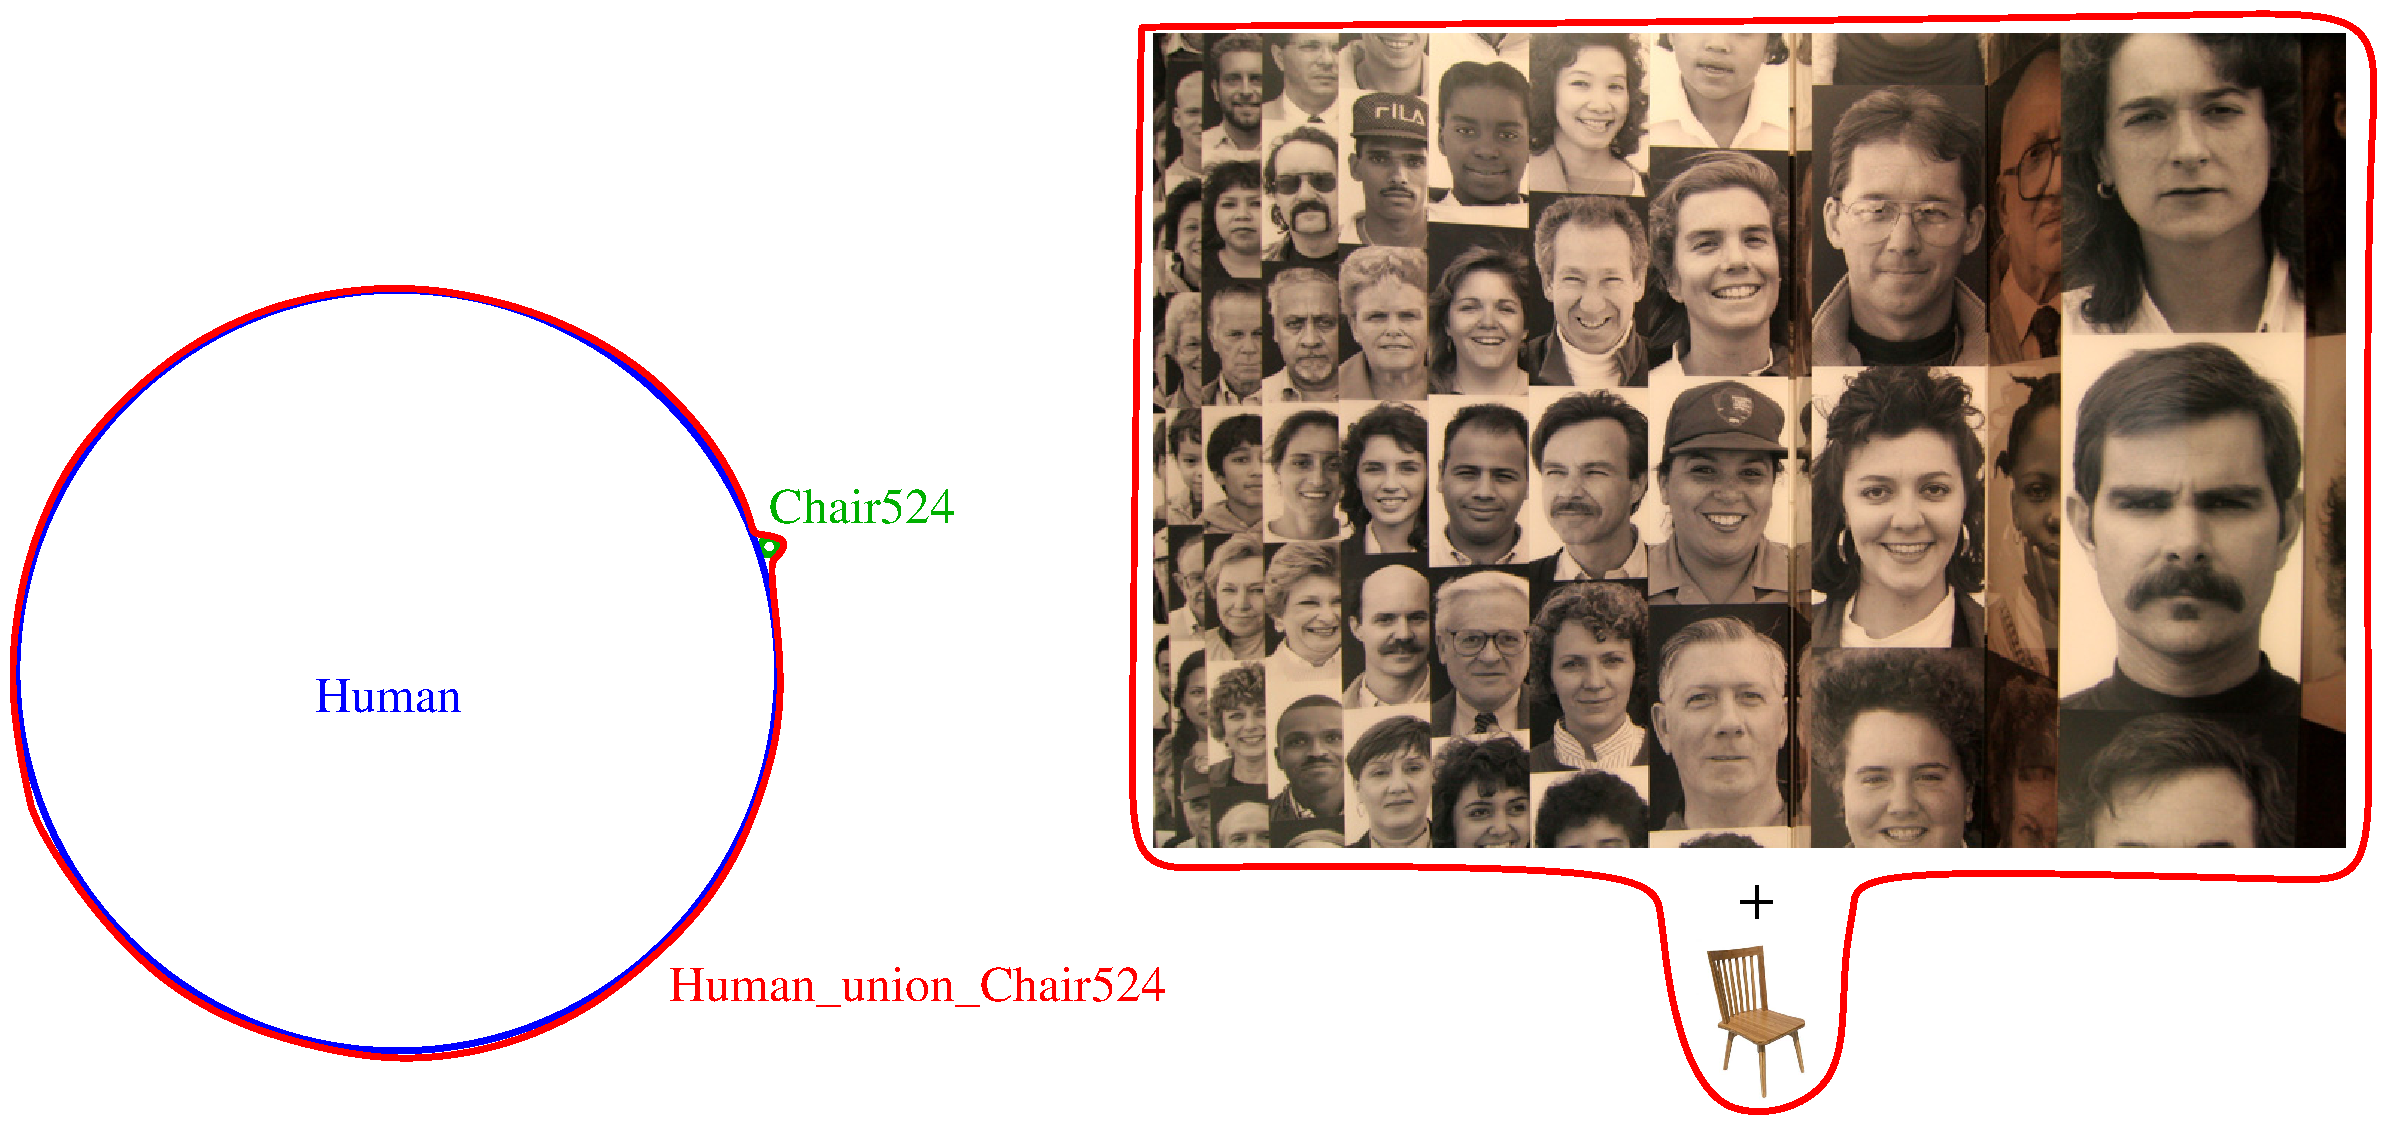
\includegraphics[scale=0.25]{human_chair_pic.pdf}}

  \visible<4>{
    \alert{$ASSOC(Human\_union\_Chair524,Human)$ is high},
    yet $Human\_union\_Chair524$ is \alert{not an interesting property}
    of Human.
  }
}

\frame
{
  \frametitle{Interesting property: \alert{Less complex} than the term itself}
  
  \begin{center}
    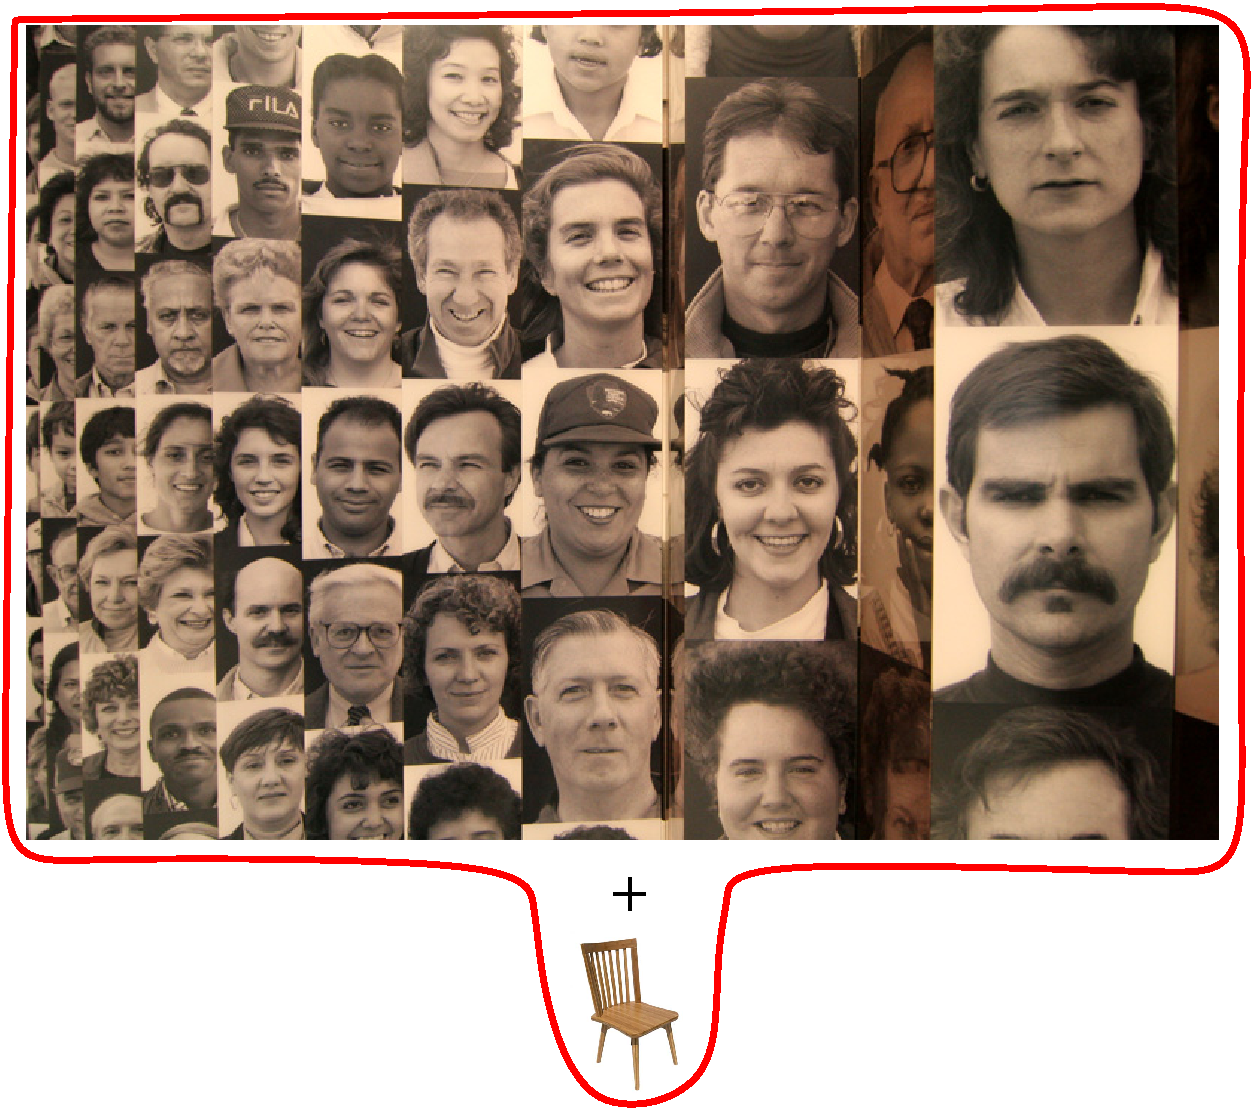
\includegraphics[scale=0.23]{hc_pic.pdf}
  \end{center}

  \begin{beamerboxesrounded}{$Human\_union\_Chair524$ is
      \alert{more complex} than Human}
    $c(Human\_union\_Chair524) \approx c(Human) + c(Chair524)$
  \end{beamerboxesrounded}
}

\frame
{
  \frametitle{Interesting property: \alert{Less complex} than the term itself}

  \begin{center}
    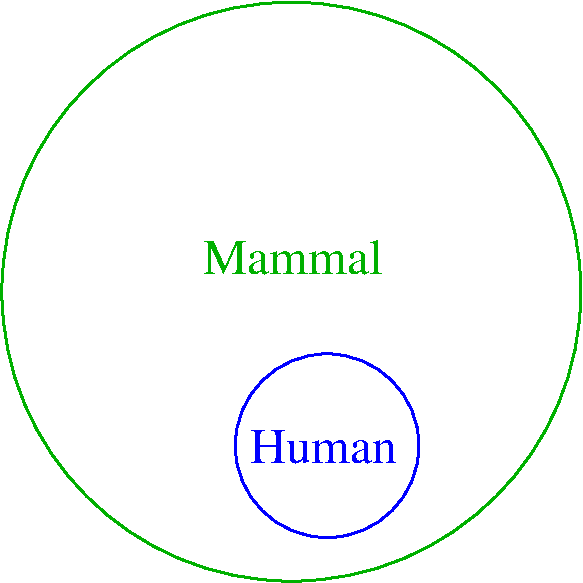
\includegraphics[scale=0.4]{mammal_human.pdf}
  \end{center}
  
  \begin{beamerboxesrounded}{Mammal is \alert{less complex} than Human,
      c(Mammal) < c(Human)}
    A human is a mammal + additional characteristics 
  \end{beamerboxesrounded}
}

\frame
{
  \frametitle{Interesting property: \alert{Less complex} than the term itself}

  \begin{beamerboxesrounded}{If $F$ is a property of $G$ we want}
    c(F)<c(G)
  \end{beamerboxesrounded}

  \[[c(G)-c(F)]^+\]
  \visible<+->{
  \visible<2->{Examples:}
  \begin{itemize}
  \item<+-> $[c(Human)-c(Human\_union\_Chair524)]^+ = 0$
  \item<+-> $[c(Human)-c(Mammal)]^+ > 0$\\[3ex]
  \end{itemize}
  }
  {\footnotesize Complexity of $F$, $c(F)$ is for example the
  shortest description of $F$ in some language $L$.}

}

\frame
{
  \frametitle{What is an \alert{interesting} property? A \alert{Pattern}}

  \begin{enumerate}
  \item Help \alert{differentiate} that term, $ASSOC(F,G)$\footnote{
      $ASSOC(F,G) = [P(F|G)-P(F|\lnot G)]^+$}

  \item \alert{Less complex} than the term itself,
    $[c(G)-c(F)]^+$
  \end{enumerate}
    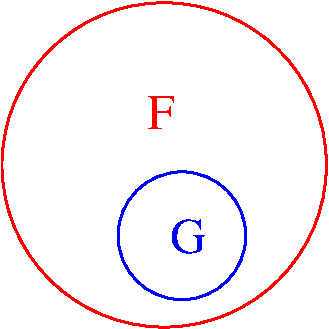
\includegraphics[scale=0.2]{F_G.pdf}  
  \pause

  \begin{beamerboxesrounded}{$F$ is a \alert{pattern} of $G$ if}
    $F$ is \alert{associated} with $G$ and $F$ is \alert{less complexe} than $G$
  \end{beamerboxesrounded}


    \[PAT(F,G)=[c(G)-c(F)]^+ \times ASSOC(F,G)\]
    
}

\frame
{
  \frametitle{Intensional Inheritance = Pattern Inheritance}

  \begin{beamerboxesrounded}{$A$ Intensionally Inherits $B$}
    \alert{How many patterns} $A$ inherits from $B$
  \end{beamerboxesrounded}
  
  \pause
  
  More formally...\\[2ex]

  Definition: $X\_PAT$ is the \alert{fuzzy set of all patterns of $X$}, that is:
  \[X\_PAT(G) = PAT(G,X)\]
 
  \pause
  
  For example:
  $
  \begin{array}{|lcc|}
    \hline
    Tiger\_PAT(Predator) & = & 0.3\\
    Tiger\_PAT(Mammal) & = & 0.4\\
    Tiger\_PAT(Carnivore) & = & 0.2\\
    Tiger\_PAT(Facing\_extinction) & = & 0.15\\
    Tiger\_PAT(Striped) & = & 0.3\\
    \hline
  \end{array}
  $
}

\frame
{
  \frametitle{Intensional Inheritance $\Rightarrow$ Extensional Inheritance}
  
  \begin{center}
    {\tt IntInh A B} $\ \ \equiv \ \ $
    {\tt ExtInh A\_PAT B\_PAT}\\
    $\equiv$\\
    {\tt SubSet A\_PAT B\_PAT}
    $\ \ = \ \  P(B\_PAT|A\_PAT)$
  \end{center}
}

\frame
{

  \frametitle{Intensional Inheritance $\Rightarrow$ Extensional Inheritance}

  For example: {\tt IntInh Tiger Lion <?>}

  \pause 

  \begin{enumerate}
  \item<+-> Determine Tiger\_PAT and Lion\_PAT

    \begin{columns}
      
      \column{1.5in}
      {\tiny
        $
        \begin{array}{|lcc|}
          \hline
          Lion\_PAT(Predator) & = & 0.3\\
          Lion\_PAT(Mammal) & = & 0.4\\
          Lion\_PAT(Carnivore) & = & 0.2\\
          Lion\_PAT(Facing\_extinction) & = & 0.1\\
          Lion\_PAT(Striped) & = & 0\\
          Lion\_PAT(Large\_Mane) & = & 0.3\\
          \hline
        \end{array}
        $
      }

      \column{1.5in}      

      {\tiny
        $
        \begin{array}{|lcc|}
          \hline
          Tiger\_PAT(Predator) & = & 0.3\\
          Tiger\_PAT(Mammal) & = & 0.4\\
          Tiger\_PAT(Carnivore) & = & 0.2\\
          Tiger\_PAT(Facing\_Extinction) & = & 0.15\\
          Tiger\_PAT(Striped) & = & 0.3\\
          Tiger\_PAT(Large\_Mane) & = & 0.01\\
          \hline
        \end{array}
        $
      }
      

  \end{columns}

  \item<+->

    {\tiny
      \begin{eqnarray*}
        P(Tiger\_PAT|Lion\_PAT)
        &
        =
        &
        \frac{\sum_x \min(Lion\_PAT(x), Tiger\_PAT(x))}
        {\sum_x Lion\_PAT(x)}\\
        \pause
        &
        =
        & 
        \frac{0.3+0.4+0.2+\min(0.1,0.15)+\min(0,0.3)+\min(0.3,0.01)}
        {0.3+0.4+0.2+0.1+0+0.3} = 0.78
      \end{eqnarray*}
    }

  \item<+->
      \alert{{\tt IntInh Lion Tiger <0.78>}}
  \end{enumerate}

}

\fi

\subsection{Level 3: Contextual Inference}

\frame
{
  \frametitle{Context is almost kinda equivalent to SubSet!}

  \begin{columns}
    \column{1.9in}

    ContextLink <TV>\\
    $\ \ \ $Concept C\\
    $\ \ \ $Concept A\\

    \column{.05in}
    
    $\equiv$
    
    \column{2in}
  
    SubSet <TV>\\
    $\ \ \ $Concept C\\
    $\ \ \ $Concept A\\
  \end{columns}

  $\ $\\[.5cm]

  \pause

  \underline{More generally} [or not]
  \begin{columns}
    \column{1.9in}

    ContextLink <TV>\\
    $\ \ \ $C\\
    $\ \ \ $R\\
    $\ \ \ $$\ \ \ $A1\\
    $\ \ \ $$\ \ \ $...\\
    $\ \ \ $$\ \ \ $An\\

    \column{.05in}
    
    $\equiv$
    
    \column{2in}
 
    $\ \ \ $R <TV>\\
    $\ \ \ $$\ \ \ $And A1 C\\
    $\ \ \ $$\ \ \ $...\\
    $\ \ \ $$\ \ \ $And An C\\
 
  \end{columns}
}

\subsection{Level 4: Sugar}

\frame
{
  \frametitle{Lambda}

  \begin{beamerboxesrounded}{Remark}
    All atoms taking place in a PLN inference chain have \alert{only
    scoped variables}.
  \end{beamerboxesrounded}

}

\frame
{
  \frametitle{Implication Sugar Syntax}

  {\scriptsize

  \begin{columns}
    \column{2in}
    \underline{Basic format}\\[.2cm]
    Implication\\
    $\ \ \ $<implicant-predicate>\\
    $\ \ \ $<implicand-predicate>\\
    \column{1.5in}
    \underline{Example}\\[.2cm]
    Implication\\
    $\ \ \ $Predicate "is-primate"\\
    $\ \ \ $Predicate "is-mammal"\\
  \end{columns}

  }
}

\frame
{
  \frametitle{Implication Sugar Syntax}

  {\tiny

  \begin{columns}
    \column{2in}
    \underline{Using Lambda}\\[.2cm]
    Implication\\
    $\ \ \ $Lambda\\
    $\ \ \ $$\ \ \ $<variables>\\
    $\ \ \ $$\ \ \ $<implicant-predicate-body>\\
    $\ \ \ $Lambda\\
    $\ \ \ $$\ \ \ $<variables>\\
    $\ \ \ $$\ \ \ $<implicand-predicate-body>\\

    \column{2in}
    \underline{Example}\\[.2cm]
    Implication\\
    $\ \ \ $TypedVariable\\
    $\ \ \ $$\ \ \ $Variable X\\
    $\ \ \ $$\ \ \ $Type "ConceptNode"\\
    $\ \ \ $Lambda\\
    $\ \ \ $$\ \ \ $TypedVariable\\
    $\ \ \ $$\ \ \ $$\ \ \ $Variable X\\
    $\ \ \ $$\ \ \ $$\ \ \ $Type "ConceptNode"\\
    $\ \ \ $$\ \ \ $Evaluation\\
    $\ \ \ $$\ \ \ $$\ \ \ $Predicate "is-primate"\\
    $\ \ \ $$\ \ \ $$\ \ \ $X\\
    $\ \ \ $Lambda\\
    $\ \ \ $$\ \ \ $TypedVariable\\
    $\ \ \ $$\ \ \ $$\ \ \ $Variable X\\
    $\ \ \ $$\ \ \ $$\ \ \ $Type "ConceptNode"\\
    $\ \ \ $$\ \ \ $Evaluation\\
    $\ \ \ $$\ \ \ $$\ \ \ $Predicate "is-mammal"\\
    $\ \ \ $$\ \ \ $$\ \ \ $X\\
  \end{columns}

  }
}
  
\frame
{
  \frametitle{Implication Sugar Syntax}

  {\tiny

  \begin{columns}
    \column{2in}
    \underline{Sugar form}\\[.2cm]
    Implication\\
    $\ \ \ $<variables>\\
    $\ \ \ $<implicant-predicate-body>\\
    $\ \ \ $<implicand-predicate-body>\\
    \column{2in}
    \underline{Example}\\[.2cm]
    Implication\\
    $\ \ \ $TypedVariable\\
    $\ \ \ $$\ \ \ $Variable X\\
    $\ \ \ $$\ \ \ $Type "ConceptNode"\\
    $\ \ \ $Evaluation\\
    $\ \ \ $$\ \ \ $Predicate "is-primate"\\
    $\ \ \ $$\ \ \ $X\\
    $\ \ \ $Evaluation\\
    $\ \ \ $$\ \ \ $Predicate "is-mammal"\\
    $\ \ \ $$\ \ \ $X\\
  \end{columns}

  }
}

\iffalse

\section{Inference and Control}

\frame
{

  \frametitle{URE}

  Inferences are performed by the \alert{Unified Rule Engine}, using
  the \alert{Forward Chainer} (already functional) and the
  \alert{Backward Chainer} (in development).\\[1cm]

}

\frame
{

  \begin{columns}

    \column{2in}

    PLN Rules are represented in the URE rule format, BindLink for the
    mandatory forward form, or possibly a list of BindLinks (forward and
    backward forms).

    \column{2in}  

{\tiny


    
  Bind\\
  $\ \ \ $Variable\\
  $\ \ \ $$\ \ \ $Variable "\$A"\\
  $\ \ \ $$\ \ \ $Variable "\$B"\\
  $\ \ \ $$\ \ \ $Variable "\$C"\\
  $\ \ \ $AndLink\\
  $\ \ \ $$\ \ \ $Implication\\
  $\ \ \ $$\ \ \ $$\ \ \ $Variable "\$A"\\
  $\ \ \ $$\ \ \ $$\ \ \ $Variable "\$B"\\
  $\ \ \ $$\ \ \ $Implication\\
  $\ \ \ $$\ \ \ $$\ \ \ $VariableNode "\$B"\\
  $\ \ \ $$\ \ \ $$\ \ \ $VariableNode "\$C"\\
  $\ \ \ $$\ \ \ $NotLink\\
  $\ \ \ $$\ \ \ $$\ \ \ $EqualLink\\
  $\ \ \ $$\ \ \ $$\ \ \ $$\ \ \ $VariableNode "\$A"\\
  $\ \ \ $$\ \ \ $$\ \ \ $$\ \ \ $VariableNode "\$C"\\
  $\ \ \ $ExecutionOutputLink\\
  $\ \ \ $$\ \ \ $GroundedSchemaNode "scm: deduction-formula"\\
  $\ \ \ $$\ \ \ $ListLink\\
  $\ \ \ $$\ \ \ $$\ \ \ $Implication\\
  $\ \ \ $$\ \ \ $$\ \ \ $$\ \ \ $VariableNode "\$A"\\
  $\ \ \ $$\ \ \ $$\ \ \ $$\ \ \ $VariableNode "\$B"\\
  $\ \ \ $$\ \ \ $$\ \ \ $Implication\\
  $\ \ \ $$\ \ \ $$\ \ \ $$\ \ \ $VariableNode "\$B"\\
  $\ \ \ $$\ \ \ $$\ \ \ $$\ \ \ $VariableNode "\$C"\\
  $\ \ \ $$\ \ \ $$\ \ \ $Implication\\
  $\ \ \ $$\ \ \ $$\ \ \ $$\ \ \ $VariableNode "\$A"\\
  $\ \ \ $$\ \ \ $$\ \ \ $$\ \ \ $VariableNode "\$C"\\

  }

  \end{columns}

}

\fi

\section{Open questions}

\frame
{
  \frametitle{Instantiation done right}

  \begin{itemize}
  \item  How reconcile instantiations from different predicates or
    implications?
    
    Suppose we have predicate Q <0.01 0.99999>\\[.2cm]
    
    And implication P->Q <0.2 0.9>\\[.2cm]
  
    One universally instantiate with A based on Q, leading to\\
    
    Q(A) <0.01 0.99999>\\[.2cm]
    
    or conditionally instantiate with A based on P->Q (assuming that
    P(A) holds), leading to\\[.2cm]
    
    Q(A) <0.2 0.9>\\[.2cm]

  \end{itemize}

}

\frame
{
  \frametitle{Priors}

  \begin{itemize}
    \item How to represent (let alone decide) a prior in a Atom? For
      instance if we have\\[0.2cm]

      Implication\\
      $\ \ \ $<very complex P>\\
      $\ \ \ $<very complex Q>\\[.2cm]
      
      we may want to use some prior to for instance \alert{decrease}
      the confidence of such an atom, or perhaps \alert{increase} its
      confidence that Q doesn't depend on P.\\[.2cm]

      Perhaps we can represent these priors in the AtomSpace itself!
      using higher order facts, etc, and just let PLN chew on them.
  \end{itemize}
}

\frame
{
  \frametitle{Objective Probabilistic Atom Semantics}

  {\tiny

  What is $\Omega$?\\[.5cm]

  Implication <TV>\\
  $\ \ \ $Evaluation\\
  $\ \ \ $$\ \ \ $Predicate "sensor-A"\\
  $\ \ \ $Evaluation\\
  $\ \ \ $$\ \ \ $Predicate "sensor-B"\\[.5cm]

  Implication <TV>\\
  $\ \ \ $Lambda\\
  $\ \ \ $$\ \ \ $Variable "\$T"\\
  $\ \ \ $$\ \ \ $AtTime "\$T"\\
  $\ \ \ $$\ \ \ $$\ \ \ $Evaluation\\
  $\ \ \ $$\ \ \ $$\ \ \ $$\ \ \ $Predicate "sensor-A"\\
  $\ \ \ $Lambda\\
  $\ \ \ $$\ \ \ $Variable "\$T"\\
  $\ \ \ $$\ \ \ $AtTime "\$T"\\
  $\ \ \ $$\ \ \ $$\ \ \ $Evaluation\\
  $\ \ \ $$\ \ \ $$\ \ \ $$\ \ \ $Predicate "sensor-B"\\[.5cm]

  So Evaluation a can be a Predicate as well. Then you don't want to
  use systematically Fuzzy TV semantics for And, Or, etc.

  }
}

\end{document}
